\documentclass[nooutcomes]{ximera}
%\documentclass[space,handout,nooutcomes]{ximera}

\usepackage{epsfig}

\graphicspath{
  {./}
  {figures/}
  {../laode}
  {../laode/figures}
}

\usepackage{epstopdf}
\epstopdfsetup{outdir=./}

\usepackage{morewrites}
\makeatletter
\newcommand\subfile[1]{%
\renewcommand{\input}[1]{}%
\begingroup\skip@preamble\otherinput{#1}\endgroup\par\vspace{\topsep}
\let\input\otherinput}
\makeatother

\newcommand{\EXER}{}
\newcommand{\includeexercises}{\EXER\directlua{dofile(kpse.find_file("exercises","lua"))}}

\newenvironment{computerExercise}{\begin{exercise}}{\end{exercise}}

%\newcounter{ccounter}
%\setcounter{ccounter}{1}
%\newcommand{\Chapter}[1]{\setcounter{chapter}{\arabic{ccounter}}\chapter{#1}\addtocounter{ccounter}{1}}

%\newcommand{\section}[1]{\section{#1}\setcounter{thm}{0}\setcounter{equation}{0}}

%\renewcommand{\theequation}{\arabic{chapter}.\arabic{section}.\arabic{equation}}
%\renewcommand{\thefigure}{\arabic{chapter}.\arabic{figure}}
%\renewcommand{\thetable}{\arabic{chapter}.\arabic{table}}

%\newcommand{\Sec}[2]{\section{#1}\markright{\arabic{ccounter}.\arabic{section}.#2}\setcounter{equation}{0}\setcounter{thm}{0}\setcounter{figure}{0}}
  
\newcommand{\Sec}[2]{\section{#1}}

\setcounter{secnumdepth}{2}
%\setcounter{secnumdepth}{1} 

%\newcounter{THM}
%\renewcommand{\theTHM}{\arabic{chapter}.\arabic{section}}

\newcommand{\trademark}{{R\!\!\!\!\!\bigcirc}}
%\newtheorem{exercise}{}

\newcommand{\dfield}{{\sf dfield9}}
\newcommand{\pplane}{{\sf pplane9}}
\newcommand{\PPLANE}{{\sf PPLANE9}}

% BADBAD: \newcommand{\Bbb}{\bf}

\newcommand{\R}{\mbox{$\Bbb{R}$}}
\newcommand{\C}{\mbox{$\Bbb{C}$}}
\newcommand{\Z}{\mbox{$\Bbb{Z}$}}
\newcommand{\N}{\mbox{$\Bbb{N}$}}
\newcommand{\D}{\mbox{{\bf D}}}
\usepackage{amssymb}
%\newcommand{\qed}{\hfill\mbox{\raggedright$\square$} \vspace{1ex}}
%\newcommand{\proof}{\noindent {\bf Proof:} \hspace{0.1in}}

\newcommand{\setmin}{\;\mbox{--}\;}
\newcommand{\Matlab}{{M\small{AT\-LAB}} }
\newcommand{\Matlabp}{{M\small{AT\-LAB}}}
\newcommand{\computer}{\Matlab Instructions}
\newcommand{\half}{\mbox{$\frac{1}{2}$}}
\newcommand{\compose}{\raisebox{.15ex}{\mbox{{\scriptsize$\circ$}}}}
\newcommand{\AND}{\quad\mbox{and}\quad}
\newcommand{\vect}[2]{\left(\begin{array}{c} #1_1 \\ \vdots \\
 #1_{#2}\end{array}\right)}
\newcommand{\mattwo}[4]{\left(\begin{array}{rr} #1 & #2\\ #3
&#4\end{array}\right)}
\newcommand{\mattwoc}[4]{\left(\begin{array}{cc} #1 & #2\\ #3
&#4\end{array}\right)}
\newcommand{\vectwo}[2]{\left(\begin{array}{r} #1 \\ #2\end{array}\right)}
\newcommand{\vectwoc}[2]{\left(\begin{array}{c} #1 \\ #2\end{array}\right)}

\newcommand{\ignore}[1]{}


\newcommand{\inv}{^{-1}}
\newcommand{\CC}{{\cal C}}
\newcommand{\CCone}{\CC^1}
\newcommand{\Span}{{\rm span}}
\newcommand{\rank}{{\rm rank}}
\newcommand{\trace}{{\rm tr}}
\newcommand{\RE}{{\rm Re}}
\newcommand{\IM}{{\rm Im}}
\newcommand{\nulls}{{\rm null\;space}}

\newcommand{\dps}{\displaystyle}
\newcommand{\arraystart}{\renewcommand{\arraystretch}{1.8}}
\newcommand{\arrayfinish}{\renewcommand{\arraystretch}{1.2}}
\newcommand{\Start}[1]{\vspace{0.08in}\noindent {\bf Section~\ref{#1}}}
\newcommand{\exer}[1]{\noindent {\bf \ref{#1}}}
\newcommand{\ans}{\textbf{Answer:} }
\newcommand{\matthree}[9]{\left(\begin{array}{rrr} #1 & #2 & #3 \\ #4 & #5 & #6
\\ #7 & #8 & #9\end{array}\right)}
\newcommand{\cvectwo}[2]{\left(\begin{array}{c} #1 \\ #2\end{array}\right)}
\newcommand{\cmatthree}[9]{\left(\begin{array}{ccc} #1 & #2 & #3 \\ #4 & #5 &
#6 \\ #7 & #8 & #9\end{array}\right)}
\newcommand{\vecthree}[3]{\left(\begin{array}{r} #1 \\ #2 \\
#3\end{array}\right)}
\newcommand{\cvecthree}[3]{\left(\begin{array}{c} #1 \\ #2 \\
#3\end{array}\right)}
\newcommand{\cmattwo}[4]{\left(\begin{array}{cc} #1 & #2\\ #3
&#4\end{array}\right)}

\newcommand{\Matrix}[1]{\ensuremath{\left(\begin{array}{rrrrrrrrrrrrrrrrrr} #1 \end{array}\right)}}

\newcommand{\Matrixc}[1]{\ensuremath{\left(\begin{array}{cccccccccccc} #1 \end{array}\right)}}



\renewcommand{\labelenumi}{\theenumi}
\newenvironment{enumeratea}%
{\begingroup
 \renewcommand{\theenumi}{\alph{enumi}}
 \renewcommand{\labelenumi}{(\theenumi)}
 \begin{enumerate}}
 {\end{enumerate}\endgroup}

\newcounter{help}
\renewcommand{\thehelp}{\thesection.\arabic{equation}}

%\newenvironment{equation*}%
%{\renewcommand\endequation{\eqno (\theequation)* $$}%
%   \begin{equation}}%
%   {\end{equation}\renewcommand\endequation{\eqno \@eqnnum
%$$\global\@ignoretrue}}

%\input{psfig.tex}

\author{Martin Golubitsky and Michael Dellnitz}

%\newenvironment{matlabEquation}%
%{\renewcommand\endequation{\eqno (\theequation*) $$}%
%   \begin{equation}}%
%   {\end{equation}\renewcommand\endequation{\eqno \@eqnnum
% $$\global\@ignoretrue}}

\newcommand{\soln}{\textbf{Solution:} }
\newcommand{\exercap}[1]{\centerline{Figure~\ref{#1}}}
\newcommand{\exercaptwo}[1]{\centerline{Figure~\ref{#1}a\hspace{2.1in}
Figure~\ref{#1}b}}
\newcommand{\exercapthree}[1]{\centerline{Figure~\ref{#1}a\hspace{1.2in}
Figure~\ref{#1}b\hspace{1.2in}Figure~\ref{#1}c}}
\newcommand{\para}{\hspace{0.4in}}

\usepackage{ifluatex}
\ifluatex
\ifcsname displaysolutions\endcsname%
\else
\renewenvironment{solution}{\suppress}{\endsuppress}
\fi
\else
\renewenvironment{solution}{}{}
\fi

%\ifxake
%\newenvironment{matlabEquation}{\begin{equation}}{\end{equation}}
%\else
\newenvironment{matlabEquation}%
{\let\oldtheequation\theequation\renewcommand{\theequation}{\oldtheequation*}\begin{equation}}%
  {\end{equation}\let\theequation\oldtheequation}
%\fi

\makeatother



\title{Midsegment Theorem}
\author{Brad Findell}
\begin{document}
\begin{abstract}
Proofs updated. 
\end{abstract}
\maketitle

\begin{definition}
In a triangle, a \emph{midsegment} is a line joining the midpoints of two sides.  
\end{definition}

\begin{theorem}
Midsegment Theorem:  A midsegment in a triangle is parallel to and half the length of the corresponding side.
\end{theorem}

\fixnote{The typical proof uses similarity, which is suitable for Math 2.  This one uses parallelograms, so that it is suitable for Math 1.}

In preparation for the midsegment theorem, the class proved some useful theorems about parallelograms. 

\begin{theorem}
Antonia's Theorem:  If the diagonals of a quadrilateral bisect each other, then the quadrilateral is a parallelogram. 
\end{theorem}

\begin{theorem}
Lu's Theorem:  If one pair of sides of a quadrilateral are congruent and parallel, then the quadrilateral is a parallelogram. 
\end{theorem}

\begin{problem}
To prove the midsegment theorem for $\triangle ABC$ with midpoints $D$ and $E$ of sides $AC$ and $BC$, respectively, Jesse extends $\overline{DE}$ to a point $X$ such that $EX=DE$, as shown in the marked figure.   
%$$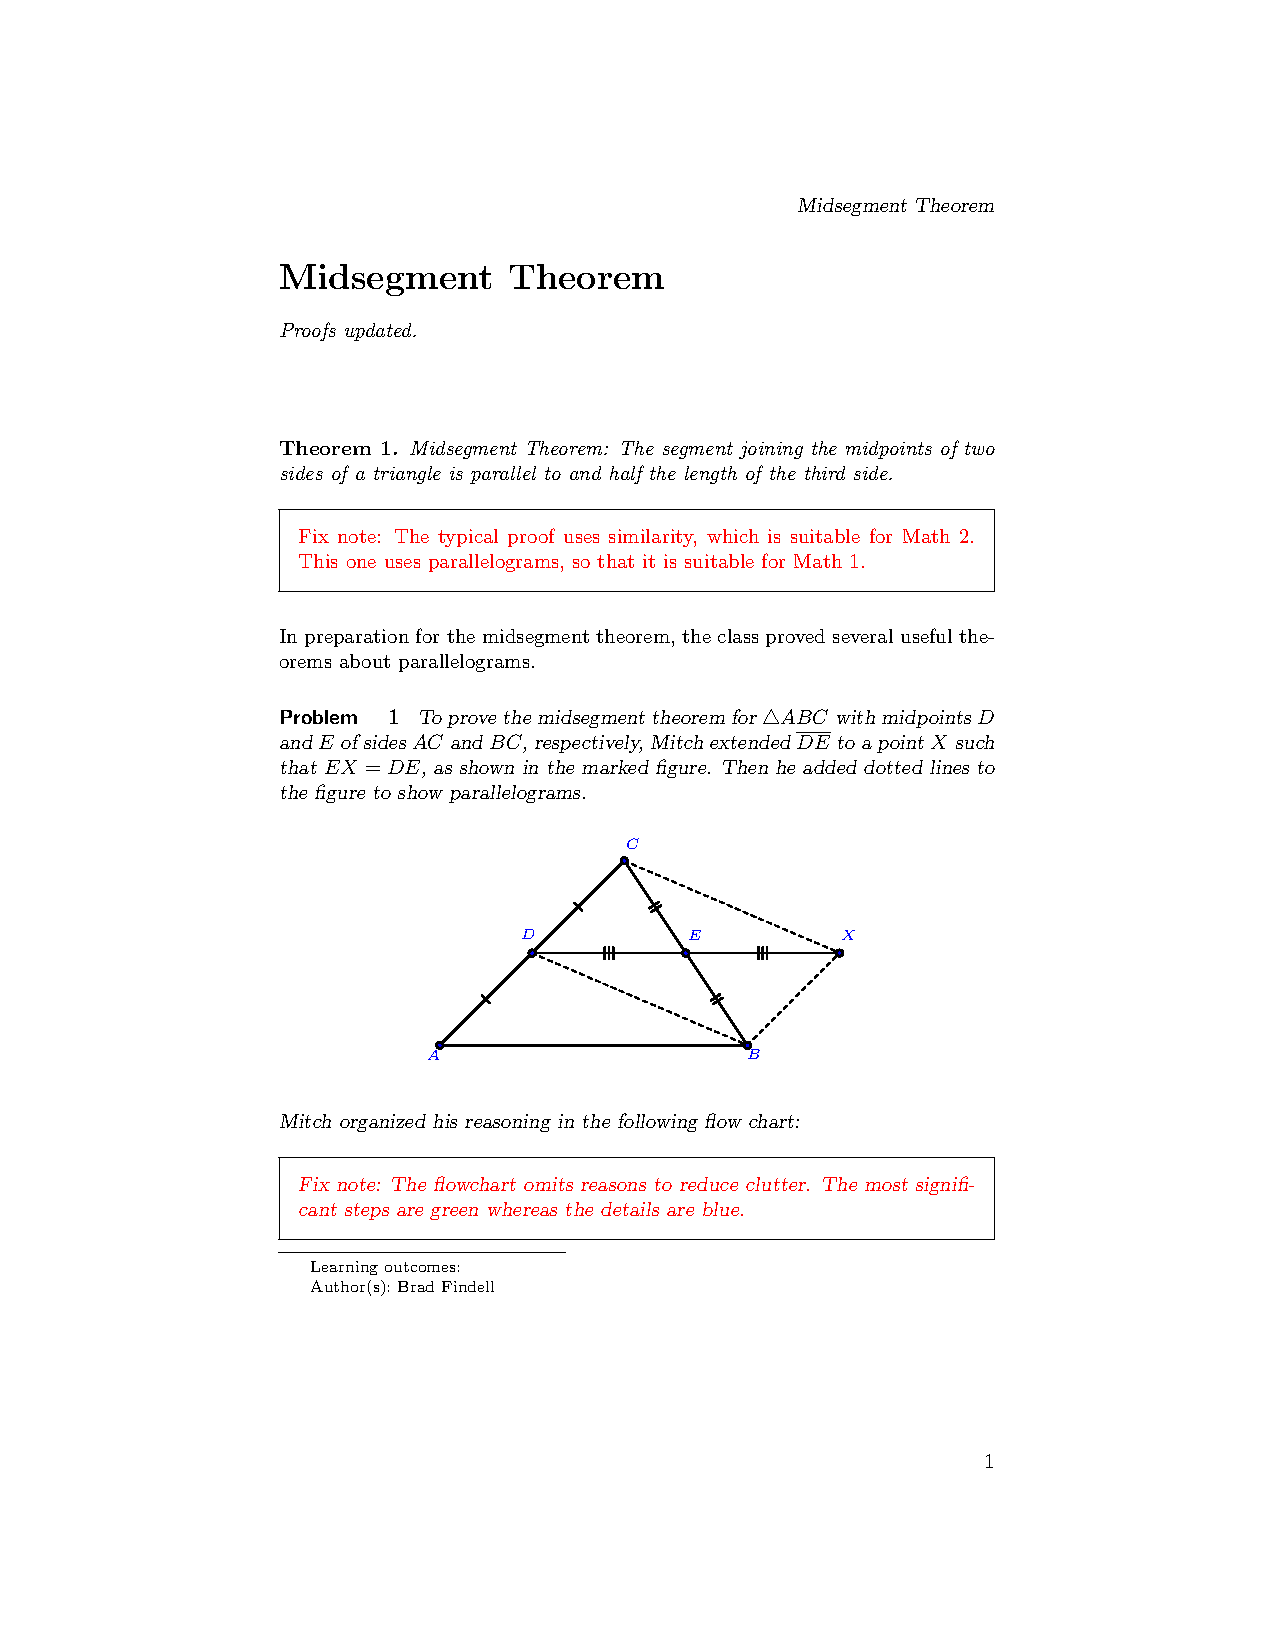
\includegraphics[scale=0.7]{../graphics/midsegment}$$

\begin{image}
\definecolor{qqqqff}{rgb}{0.,0.,1.}
\begin{tikzpicture}[line width=0.8pt,line cap=round,line join=round,>=triangle 45,x=1.0cm,y=1.0cm]
\clip(-0.34,-0.44) rectangle (6.86,3.4);
\draw (5.,0.)-- (0.,0.);
\draw (0.,0.)-- (1.5,1.5);
\draw (0.686,0.814) -- (0.814,0.686);
\draw (1.5,1.5)-- (3.,3.);
\draw (2.186,2.314) -- (2.314,2.187);
\draw (1.5,1.5)-- (4.,1.5);
\draw (2.68,1.59) -- (2.68,1.41);
\draw (2.75,1.59) -- (2.75,1.41);
\draw (2.82,1.59) -- (2.82,1.41);
\draw (4.,1.5)-- (6.5,1.5);
\draw (5.18,1.59) -- (5.18,1.41);
\draw (5.25,1.59) -- (5.25,1.41);
\draw (5.32,1.59) -- (5.32,1.41);
\draw (3.,3.)-- (4.,1.5);
\draw (3.555,2.329) -- (3.406,2.229);
\draw (3.594,2.271) -- (3.444,2.171);
\draw (4.,1.5)-- (5.,0.);
\draw (4.555,0.829) -- (4.406,0.729);
\draw (4.594,0.771) -- (4.445,0.671);
\draw [line width=0.6pt,dash pattern=on 2pt off 2pt] (5.,0.)-- (6.5,1.5);
\draw [line width=0.6pt,dash pattern=on 2pt off 2pt] (3.,3.)-- (6.5,1.5);
\draw [line width=0.6pt,dash pattern=on 2pt off 2pt] (1.5,1.5)-- (5.,0.);
\begin{scriptsize}
\draw [fill=qqqqff] (0.,0.) circle (1.5pt);
\draw[color=qqqqff] (-0.1,-0.15) node {$A$};
\draw [fill=qqqqff] (5.,0.) circle (1.5pt);
\draw[color=qqqqff] (5.1,-0.13) node {$B$};
\draw [fill=qqqqff] (3.,3.) circle (1.5pt);
\draw[color=qqqqff] (3.14,3.27) node {$C$};
\draw [fill=qqqqff] (6.5,1.5) circle (1.5pt);
\draw[color=qqqqff] (6.64,1.79) node {$X$};
\draw [fill=qqqqff] (1.5,1.5) circle (1.5pt);
\draw[color=qqqqff] (1.44,1.81) node {$D$};
\draw [fill=qqqqff] (4.,1.5) circle (1.5pt);
\draw[color=qqqqff] (4.14,1.79) node {$E$};
\end{scriptsize}
\end{tikzpicture}
\end{image}

Jesse organizes her reasoning in the following flow chart:  
\fixnote{The flowchart omits reasons to reduce clutter.  The most significant steps are green whereas the details are blue.}

\begin{image}
\tikzstyle{block} = [rectangle, draw, fill=blue!20, 
    text width=6em, text centered, rounded corners, minimum height=2em]
\tikzstyle{Block} = [rectangle, draw, fill=green!20, 
    text width=10em, text centered, rounded corners, minimum height=3em]
\tikzstyle{implies} = [draw, -latex']

\begin{tikzpicture}[node distance = 1.5cm, auto]
    % Place nodes
    \node [Block] (a) {Quad. $CDBX$ is a parallelogram};
    \node [block, left of=a, node distance = 3.5cm] (init) {$CE = BE$\\$DX=EX$};
    \node [block, below of=a] (b) {$XB=CD$};
    \node [block, left of=b, node distance = 3.5cm] (init2) {$CD=AD$};
    \node [block, below of=b] (c) {$XB=AD$};
    \node [block, right of=b, node distance = 3.5cm] (d) {$\overline{XB} \parallel \overline{CD}$};
    \node [block, below of=d] (e) {$\overline{XB} \parallel \overline{AD}$};
    \node [Block, below of=c] (f) {Quad. $DABX$ is a parallelogram};
    \node [block, below of=f] (g) {$\overline{DX} \parallel \overline{AB}$};
    \node [block, below of=g] (h) {$\overline{DE} \parallel \overline{AB}$};
    \node [block, right of=f, node distance = 3.5cm] (i) {$AB = DX$};
    \node [block, text width=12em, right of=i, node distance = 4cm] (j) {$DX = DE + EX = 2DE$};
    \node [block, below of=i] (k) {$AB = 2DE$};
    \node [block, below of=k] (l) {$DE = \frac{1}{2}AB$};
    \node [Block, text width=12em, below of=h] (m) 
       {Summary: $\overline{DE}$ is parallel to $\overline{AB}$ and half its length.};    
      % Draw edges
    \path [implies] (init) -- (a);
    \path [implies] (a) -- (b);
    \path [implies] (init2) -- (c);
    \path [implies] (b) -- (c);
    \path [implies] (a) -- (d);
    \path [implies] (d) -- (e);
    \path [implies] (c) -- (f);
    \path [implies] (e) -- (f);
    \path [implies] (f) -- (g);
    \path [implies] (g) -- (h);
    \path [implies] (f) -- (i);
    \path [implies] (i) -- (k);
    \path [implies] (j) -- (k);
    \path [implies] (k) -- (l);
    \path [implies] (h) -- (m);
    \path [implies] (l) -- (m);
\end{tikzpicture}
\end{image}

\fixnote{For the following questions, does it help to name the theorems?  Would theorem numbers be better?  Or maybe we should write each theorem in words.}
In the proof above, why may Jesse conclude that quadrilateral $CDBX$ a parallelogram?  
\begin{multipleChoice}
\choice{By the Pythagorean Theorem.}
\choice{By Lu's Theorem.}
\choice[correct]{By Antonia's Theorem.}
\choice{By the Parallelogram Theorem.}
\end{multipleChoice}

In the proof above, why may Jesse conclude that quadrilateral $DABX$ a parallelogram?  
\begin{multipleChoice}
\choice{By the Pythagorean Theorem.}
\choice[correct]{By Lu's Theorem.}
\choice{By Antonia's Theorem.}
\choice{By the Parallelogram Theorem.}
\end{multipleChoice}

\detail{Paragraph proof:
\\ $CE = BE$ and $DX=EX$, as given.
\\ Quadrilateral $CDBX$ is a parallelogram by Antonia's Theorem. 
\\ $XB=CD$ because opposite sides of a parallelogram are congruent.
\\ $XB=AD$ because they are both equal to $CD$. 
\\ $\overline{XB} \parallel \overline{CD}$ because CDBX is a parallelogram. 
\\ $\overline{XB} \parallel \overline{AD}$ because $A$, $C$, and $D$ are collinear. 
\\ Quadrilateral $DABX$ is a parallelogram by Lu's Theorem.  
\\ $\overline{DX} \parallel \overline{AB}$ because $DABX$ is a parallelogram. 
\\ $\overline{DE} \parallel \overline{AB}$ because $D$, $E$, and $X$ are collinear.  
\\ $AB = DX = DE + EX = 2DE$
\\ $DE = \frac{1}{2}AB$
\\ Summary:  $DE$ is parallel to $AB$ and half its length.  
}
\end{problem}


\end{document}

